\documentclass[oneside, 11pt]{article}

\usepackage[T1]{fontenc}
\usepackage[utf8]{inputenc}
\usepackage[english]{babel}
\usepackage{enumerate}
\usepackage{isotope}


\usepackage{fouriernc}
\usepackage[detect-all, binary-units, separate-uncertainty=true,
            per-mode=symbol, retain-explicit-plus, retain-unity-mantissa=false]{siunitx}

\usepackage{setspace}
\setstretch{1.2}

\setlength{\parskip}{\smallskipamount}
\setlength{\parindent}{0pt}

\usepackage[headheight=14pt]{geometry}
\geometry{marginparwidth=0.5cm, verbose, a4paper, tmargin=3cm, bmargin=3cm,
          lmargin=2cm, rmargin=2cm}

\usepackage{float}

\usepackage[fleqn]{amsmath}
\numberwithin{equation}{section}
\numberwithin{figure}{section}

\usepackage{graphicx}
\graphicspath{{images/}{../../../images/}}

\usepackage{tikz}
\usetikzlibrary{shapes}
\usetikzlibrary{plotmarks}

\newcounter{Exercise}
\setcounter{Exercise}{1}
\usepackage{xcolor}
\definecolor{shadecolor}{gray}{0.9}
\usepackage{framed}
\usepackage{caption}

\usepackage{url}


\usepackage{fancyhdr}
\pagestyle{fancy}
\fancyhf{}
\rhead{\thepage}
\renewcommand{\footrulewidth}{0pt}
\renewcommand{\headrulewidth}{0pt}

\fancypagestyle{firststyle}
{
    \fancyhf{}
    \rhead{\thepage}
    \cfoot{\includegraphics[height=30pt]{HiSPARClogo}}
    \rfoot{\includegraphics[height=25pt]{CCbysa}}
    \lfoot{
\includegraphics[height=30pt]{NIKHEFlogo}}
    \renewcommand{\footskip}{50pt}
    \renewcommand{\footrulewidth}{0.1pt}
    \renewcommand{\headrulewidth}{0pt}
}

\newcommand{\figref}[1]{Figuur~\ref{#1}}

\newcommand{\hisparc}{\textsmaller{HiSPARC}\xspace}
\newcommand{\kascade}{\textsmaller{KASCADE}\xspace}
\newcommand{\sapphire}{\textsmaller{SAPPHiRE}\xspace}
\newcommand{\jsparc}{\textsmaller{jSparc}\xspace}
\newcommand{\hdf}{\textsmaller{HDF5}\xspace}
\newcommand{\aires}{\textsmaller{AIRES}\xspace}
\newcommand{\csv}{\textsmaller{CSV}\xspace}
\newcommand{\python}{\textsmaller{PYTHON}\xspace}
\newcommand{\corsika}{\textsmaller{CORSIKA}\xspace}
\newcommand{\labview}{\textsmaller{LabVIEW}\xspace}
\newcommand{\daq}{\textsmaller{DAQ}\xspace}
\newcommand{\adc}{\textsmaller{ADC}\xspace}
\newcommand{\hi}{\textsc{h i}\xspace}
\newcommand{\hii}{\textsc{h ii}\xspace}
\newcommand{\mip}{\textsmaller{MIP}\xspace}
\newcommand{\hisparcii}{\textsmaller{HiSPARC II}\xspace}
\newcommand{\hisparciii}{\textsmaller{HiSPARC III}\xspace}

\DeclareSIUnit{\electronvolt}{\ensuremath{\mathrm{e\!\!\:V}}}

\DeclareSIUnit{\unitsigma}{\ensuremath{\sigma}}
\DeclareSIUnit{\mip}{\textsmaller{MIP}}
\DeclareSIUnit{\adc}{\textsmaller{ADC}}

\DeclareSIUnit{\gauss}{G}
\DeclareSIUnit{\parsec}{pc}
\DeclareSIUnit{\year}{yr}



\begin{document}

\title{Krachten binnen het standaardmodel}
\author{N.G. Schultheiss}
\date{}

\maketitle
\thispagestyle{firststyle}

\section{Inleiding}

Deze module volgt op de module ``Deeltjes binnen het standaardmodel''
en wordt vervolgd met de module ``Deeltjes in airshowers''. Aan
de hand van het neutron verval bekijken we wat er op verschillende
niveau's met de deeltjes binnen het standaardmodel gebeurt. Deze deeltjes
oefenen ook krachten op elkaar uit, er is dus sprake van een wisselwerking.


\section{Krachten}

Mensen worden op aarde gehouden door de zwaartekracht. Deze is te
beschrijven met:

\begin{equation}
F_{gravitatie}=G\frac{m_{1}m_{2}}{r^{2}}
\end{equation}


Electronen worden aan een kern gebonden door de elektrische kracht.
De elektrische kracht is veel sterker dan de zwaartekracht en is te
beschrijven met:

\begin{equation}
F_{elektrisch}=\frac{1}{4\pi\varepsilon_{0}}\frac{q_{1}q_{2}}{r^{2}}
\end{equation}


\paragraph*{Opdracht 1:}

\emph{Vergelijk de grootte van de gravitatieconstante G en de diëlektrische
constante $\varepsilon_{0}$. Welke gevolgen heeft dit voor de gravitatiekracht
en de elektrische kracht?}

Het verval van een isotoop gaat met behulp van de zwakke kernkracht
of de zwakke wisselwerking. De zwakke wisselwerking maakt het quarks
mogelijk van smaak te veranderen.

In de kern werkt ook een kracht om de de protonen en neutronen bij
elkaar te houden, de sterke kernkracht. Deze sterke kernkracht is
overigens veel sterker dan de elektrische kracht. Verder wordt de
kracht groter als de kerndeeltjes verder uit elkaar komen. De quarks
binnen een hadron moeten ook bij elkaar worden gehouden, dit gebeurt
ook met de sterke kernkracht.


\section{Neutron verval}

Neutronen zijn geen stabiele deeltjes maar vervallen volgens de reactie:

\begin{equation}
_{0}^{1}n=_{1}^{1}p+_{-1}^{0}e+_{0}^{0}\bar{\nu}
\end{equation}


In deze reactievergelijking zijn al een aantal eigenschappen te herkennen: 
\begin{itemize}
\item Het aantal kerndeeltjes (baryonen) blijft gelijk.
\item Het aantal andere deeltjes (leptonen) blijft gelijk. Het ontstaan
van een elektron $\left(_{-1}^{0}e\right)$ wordt gekoppeld aan het
ontstaan van een anti-neutrino $\left(_{0}^{0}\bar{\nu}\right)$.
Deze heffen elkaar op zodat er links en rechts netto geen leptonen
zijn.
\item De lading blijft links en rechts hetzelfde. Links is het neutron elektrisch
neutraal. Rechts zijn het proton en het elektron (en het anti-neutrino)
samen neutraal.
\end{itemize}
Dit is ook in een Feynman-diagram voor te stellen:

\begin{figure}[h]
\noindent \begin{centering}
\includegraphics[scale=0.75]{feynman1}
\par\end{centering}

\caption{Een eerste Feynman-diagram voor neutron verval}
\end{figure}


In dit diagram is een nieuw deeltje te zien. Dit deeltje staat bekend
als een $\mathrm{W}^{-}$-boson. Het neutron wordt nu omgezet in een
proton, omdat een neutron een quarkcombinatie ddu heeft en het proton
een quarkcombinatie duu, kunnen we zeggen dat het d-quark onder uitzending
van het $\mathrm{W}^{-}$-boson een u-quark wordt. Het $\mathrm{W}^{-}$-boson
valt vervolging uit elkaar in een elektron en een anti-neutrino. 

Als we de tijd van links naar rechts laten gaan, reizen het neutron,
het proton en het elektron met de tijd mee. Het anti-neutrino reist
tegen de tijd in. Dit is ook te interpreteren als een deeltje dat
uit het niets verdwijnt. Er blijft een anti-deeltje over.

We kunnen de tijd ook van rechts naar links laten gaan. Een neutrino
botst nu op een anti-elektron. De lading van het elektron wordt omgekeerd
als het tegen de tijd inreist. Op vergelijkbare wijze zal de lading
van het $\mathrm{W}^{-}$-boson worden omgekeerd, Dit wordt een $\mathrm{W}^{+}$-boson.
Het $\mathrm{W}^{+}$-boson botst op een anti-proton, met een negatieve
lading, en er ontstaat een anti-neutron. Dit is een mogelijke reactie.

Als de tijd van boven naar beneden gaat botst een neutron op een anti-proton.
Er ontstaat een $\mathrm{W}^{+}$-boson omdat een anti-neutron positief
is. Het $\mathrm{W}^{+}$-boson valt uit elkaar in een neutrino en
een anti-elektron. Op het eerste gezicht lijkt dit een mogelijke reactie.
In de module ``Deeltjes binnen het standaardmodel'' hebben we echter
gezien dat een proton als een udd-quarkcombinatie kan worden geschreven.
Een neutron is een uud-quarkcombinatie. We hebben nu opeens wat quarks
over. Als we in het Feynman-diagram quarks gebruiken in plaats van
protonen en neutronen, kunnen we de tijd in iedere richting laten
lopen.

\begin{figure}[H]
\noindent \begin{centering}
\includegraphics[scale=0.75]{feynman2}
\par\end{centering}

\caption{Een beter Feynman-diagram}
\end{figure}
Naast het $\mathrm{W}^{-}$- en $\mathrm{W}^{+}$-boson is er ook
een neutraal $\mathrm{Z}$-boson. Het $W^{-}$-boson kan bijvoorbeeld
vervallen in een elektron en een anti-neutrino of een quark en een
anti-quark. De quarks hebben een verschillende lading ($-\frac{1}{3}\mathrm{e}$
en $-\frac{2}{3}\mathrm{e}$). In plaats van een elektron kan er natuurlijk
ook een muon of tau ontstaan.

Bij een $\mathrm{W}^{+}$-boson is alles andersom. 

Het $Z$-boson kan vervallen in een lepton en een antilepton (met
tegengestelde lading of beide zonder lading) of een quark en een anti-quark
(uiteraard hebben deze een tegengestelde lading). De $W^{+}$- , $W^{-}$-
of $Z$-bosonen kunnen de quarks dus als het ware van smaak veranderen.


\section{Krachten in de kern}

In het vorige hoofdstuk hebben we gezien hoe het verval van een neutron
naar een proton verloopt onder uitzending van een $\mathrm{W}^{-}$-boson.
Dit $\mathrm{W}^{-}$-boson is te beschouwen als een drager van de
zwakke kernkracht. Als we ons deze reactie voorstellen met quarks,
ontstaat het volgende schema:

\begin{figure}[h]
\noindent \begin{centering}
\includegraphics[scale=0.75]{neutronquarkverval}
\par\end{centering}

\caption{\label{fig:Het-neutronverval-op}Het neutronverval op het quark /
antiquark niveau}
\end{figure}


Het valt op dat de plaats van het $\mathrm{W}^{-}$-boson wordt ingenomen
door een $\mathrm{u\bar{d}}$-deeltje. Dit deeltje staat bekend als
een $\pi^{-}$ of een negatief pion. In eerste instantie dacht men
dat het pion verantwoordelijk was voor het verval van neutronen en
de zwakke kernkracht.

Een pion hoort bij een hele nieuwe groep deeltjes, de mesonen. Zoals
te zien is, zijn mesonen samengestelde deeltjes waarin quark anti-quark
paren zitten. Mesonen maken dus ook deel uit van de bosonen.

Voordat men aan de zoektocht naar het $\mathrm{W}^{-}$-boson begon,
moest een ander probleem worden opgelost. In de kern zitten protonen,
we kunnen ons dus afvragen waarom de protonen niet de kern uitvliegen.
Toen men het pion had ontdekt, dacht men de oorzaak van het aan elkaar
plakken van protonen gevonden te hebben. Hideki Yukawa (1907 - 1981)
volgde de redenering:
\begin{itemize}
\item De elektrische kracht is gequantiseerd voor te stellen wanneer we
de elektrische kracht verpakken in fotonen. Ieder foton draagt een
deel van de elektrische kracht. 
\item Omdat een foton een heeltallige spin heeft maakt dit deeltje overigens,
net als het pion, deel uit van de verzameling bosonen.
\item Een Bose-Einstein condensaat voegt een groep deeltjes samen tot een
quantummechanisch geheel. Misschien is een eigenschap van bosonen
dus dat ze dingen samenvoegen.
\item De kracht tussen de protonen en neutronen kan in bosonen worden verpakt.
Misschien worden alle krachten zelfs in bosonen verpakt.
\item Volgens het onzekerheidsprincipe van Heisenberg ($\triangle E\triangle t>\hbar$)
kunnen we of de energie ($\triangle E$) of de tijd ($\triangle t$)
precies meten. Het is niet mogelijk om beide tegelijk te kennen.
\item Het is dus mogelijk om gedurende korte tijd ($\triangle t$) energie
($\triangle E$) te lenen, zolang $\triangle E\triangle t<\hbar$.
Dit is namelijk nooit te meten.
\item Volgens $E=mc^{2}$ kan deze energie worden omgezet in een kortlevend
deeltje dat op een pion lijkt.
\end{itemize}
\begin{figure}[h]
\noindent \begin{centering}
\includegraphics[scale=0.75]{kernkracht}
\par\end{centering}

\caption{\label{fig:Geleende-energie-bij}Geleende energie bij een proton}
\end{figure}


Zoals in igref{fig:Geleende-energie-bij} te zien is, wordt de aan
een proton geleende energie omgezet in een nieuw kortlevend deeltje.
Omdat het deeltje weer snel moet verdwijnen, kan het niet te ver reizen
voordat het door een ander kerndeeltje (zie
\figref{fig:Het-neutronverval-op}) wordt geabsorbeerd. Het deeltje werkt
volgens deze redenering inderdaad als een soort kracht. 

Pionen zijn er in drie soorten: $\pi^{+}$, $\pi^{-}$ en $\pi^{0}$
en bestaan uit up-, down, anti-up en anti-down quarks. Omdat de combinatie
van zowel een up- en een anti-up quark en een down en een anti-down
quark geen lading heeft, is dit het $\pi^{0}$-deeltje.


\paragraph*{Opdracht 2:}

\emph{Beredeneer hoe het $\pi^{-}$- en $\pi^{0}$-deeltje samengesteld
kunnen zijn. (De eigenschappen van quarks / anti-quarks zijn in de
module ``Deeltjes binnen het standaardmodel'' te vinden.) }


\paragraph*{Opdracht 3:}

\emph{Bereken de levensduur van een pion als je weet dat $\hbar=1,0545*10^{-34}\mathrm{Js}$
is en een pion een massa van ongeveer $135\mathrm{\frac{MeV}{c^{2}}}$
voor een }$\pi^{0}$\emph{ en $140\mathrm{\frac{MeV}{c^{2}}}$ voor
een }$\pi^{+}$of $\pi^{-}$\emph{ heeft. Hoeveel energie moet er
geleend worden? Hoelang kan deze energie maximaal geleend worden als
je rekening houdt met het onzekerheidsprincipe van Heisenberg?}


\paragraph*{Opdracht 4:}

\emph{Bereken hoever het pion kan komen als het met de lichtsnelheid
zou kunnen bewegen.}

Als we de samenstelling van een $\pi^{0}$-deeltje op het internet
opzoeken, vinden we $\frac{\mathrm{u\bar{u}+d\bar{d}}}{\sqrt{2}}$.
Blijkbaar kunnen we deze samenstelling zien als twee mogelijke samenstellingen
die loodrecht op elkaar staan. Delen door $\sqrt{2}$ zorgt er dan
voor dat we weer één gemiddeld deeltje hebben.

\begin{figure}[h]
\noindent \begin{centering}
\includegraphics[scale=0.75]{wz}
\par\end{centering}

\caption{De kracht tussen baryonen als meson-uitwisseling}
\end{figure}


\section{De sterke kernkracht}

In hadronen zitten geladen quarks / antiquarks, we kunnen ons dus
afvragen waarom hadronen niet uit elkaar vliegen. De twee up-quarks
in een proton willen door de elektrische kracht veel harder uit elkaar
vliegen dan dat het down-quark ze kan vasthouden. 

Een tweede probleem is dat quarks als fermionen te beschouwen zijn. De
quarks kunnen dus niet in dezelfde quantumtoestand zitten. We hebben een
nieuwe quantiseerbare eigenschap nodig. Omdat er drie quarks /
anti-quarks in een baryon en een quark anti-quark paar in een meson
zitten zijn er 6 mogelijke toestanden voor ieder quark. Toevallig zijn
er ook zes kleuren, deze toestanden worden dan ook met kleuren
\footnote{Rood, groen, blauw, anti-rood, anti-groen en anti-blauw.}
aangeduid. Als men rood, blauw en groen licht samenvoegd ontstaat wit.
Op een vergelijkbare manier kan men een rood, een groen en een blauw
quark samenvoegen. Het totaal is dan wit. Op deze wijze zijn baryonen
samen te stellen. Om een meson samen te stellen kunnen we bijvoorbeeld
een rood en een anti-rood quark gebruiken. Het geheel is nu ook wit.

Protonen en ook neutronen worden samengehouden met kleurkrachten,
deze kleuren worden constant uitgewisseld. Een rood quark kan rood
uitzenden. Als dit quark groen wordt, wordt ook anti-groen uit\-gezonden,
het gluon is dan rood / anti-groen. Dit gluon reageert met andere
gluonen of een groene quark dat rood wordt.

\begin{figure}[H]
\noindent \begin{centering}
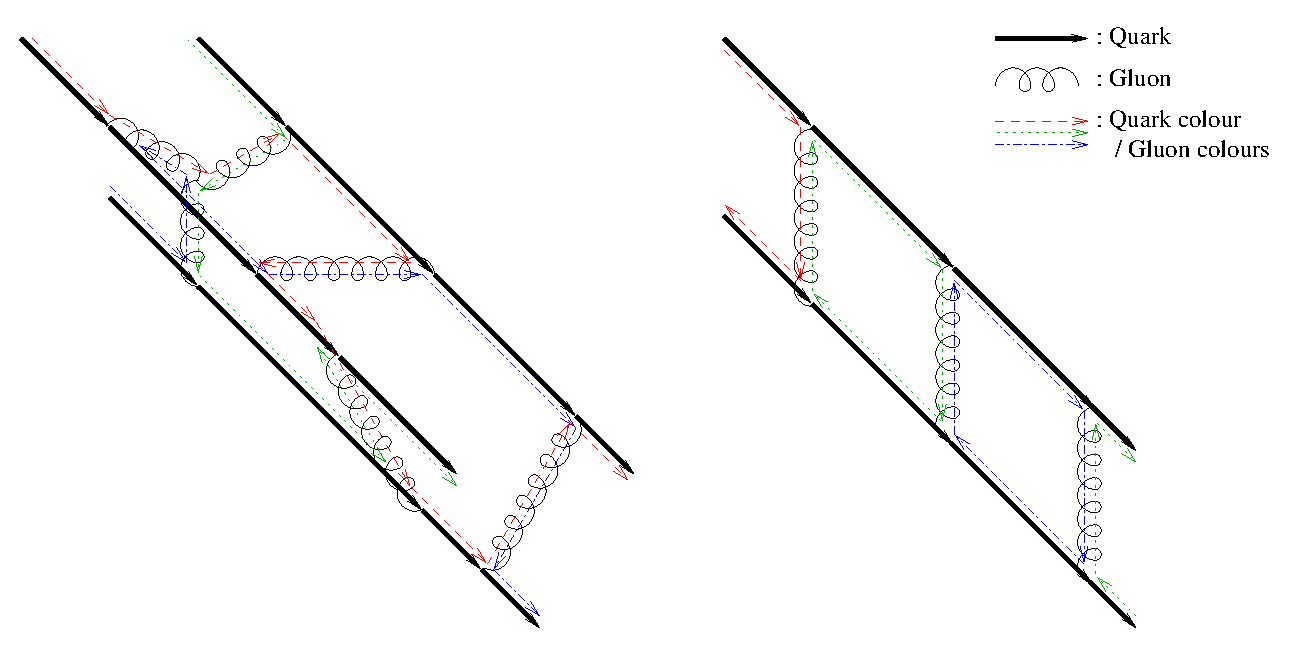
\includegraphics[scale=0.75]{gluon1}
\par\end{centering}

\caption{Gluonen in baryonen en mesonen}
\end{figure}


Omdat gluonen bosonen zijn, geldt het uitsluitingsprincipe van Pauli
niet. Gluonen kunnen dus op elkaar gestapeld worden. Verder is de
richting van het gluon onbekend, het kan net zo goed een $\mathrm{r\bar{g}}$-
als een $\mathrm{\bar{r}g}$-gluon zijn. Het gluon is nu te schrijven
als $\frac{\mathrm{r\bar{g}+\bar{r}g}}{\sqrt{2}}$. Naast dit gluon
kunnen ook alle andere kleurcombinaties worden gemaakt. Als er drie
kleuren (rood, groen, blauw) met twee toestanden (bijvoorbeeld rood
en antirood) zijn, komen we op acht ($2^{3}$) mogelijke combinaties.
Vijf daarvan zijn reëel en drie imaginair. Er bestaan overigens hypothetische
hadronen die louter uit gluonen bestaan, de ``glueballs''. Deze
zijn (nog) niet (als zodanig) aangetoond.

\begin{figure}[h]
\noindent \begin{centering}
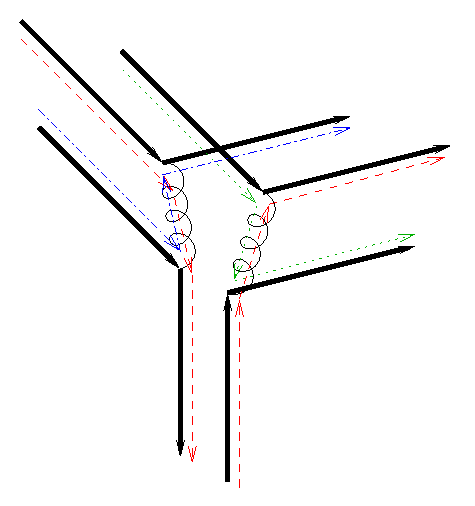
\includegraphics[scale=0.75]{gluon2}
\par\end{centering}

\caption{Baryon / meson interactie met gluonen}
\end{figure}


Een baryon kan vervallen in een lichter baryon en een meson. Tot slot
kan een baryon ook een $W^{+}$- , $W^{-}$- of $Z$-boson uitzenden
en vervallen.

\end{document}
